\newpage

\section{Przypadki testowe} \ \ \

Zostało przygotowanych 11 przykładowych przypadki testowe, które mogłyby być w zestawie testów regresyjnych dla przedstawionej aplikacji webowej. Są to zarówno przypadki pozytywne, czyli sprawdzające podstawowe funkcjonalności oprogramowania, jak i negatywne - weryfikujące zachowania się systemu w przypadku obsługi sytuacji wyjątkowych, takich jak nieprawidłowe dane.

\begin{longtable}{|l|l|
>{\columncolor[HTML]{67FD9A}}l |}
\caption{Przypadki testowe}
\label{my-label}\\
\hline
\cellcolor[HTML]{EFEFEF}\textbf{Nazwa testu} & \cellcolor[HTML]{EFEFEF}\textbf{Kroki} & \cellcolor[HTML]{EFEFEF}\textbf{Status} \\ \hline
\endfirsthead
%
\endhead
%
\begin{tabular}[c]{@{}l@{}}TC\_LogIn\_\\ LogOut\end{tabular} & \begin{tabular}[c]{@{}l@{}}1. Otwarcie przeglądarki i przekierowanie na stronę\\ https://wordpress.com/\\ 2. Logowanie do WordPress z kontem testowym.\\ 3. Po udanym zalogowaniu się, następuje \\ wylogowanie się.\\ 4. Zamknięcie przeglądarki.\end{tabular} & \multicolumn{1}{c|}{\cellcolor[HTML]{67FD9A}OK} \\ \hline
\begin{tabular}[c]{@{}l@{}}TC\_Add\_\\ Comment\end{tabular} & \begin{tabular}[c]{@{}l@{}}1. Otwarcie przeglądarki i przekierowanie na stronę\\ https://automationtestingwithjmeter.wordpress.com\\ 2. Napisanie komentarza pod postem.\\ 3. Przekierowanie na stronę https://wordpress.com/\\ 4. Logowanie do WordPress z kontem testowym.\\ 5. Przejście do strony Moja Witryna i wciśnięcie\\ przycisku Komentarze.\\ 6. Zatwierdzenie komentarza.\\ 7. Przekierowanie na bloga -\\ sprawdzenie, czy pojawił się komentarz na stronie.\\ 8. Powtórzenie kroków 3, 4 i 5.\\ 9. Usunięcie komentarza.\\ 10. Wylogowanie się.\\ 11. Przekierowanie na bloga -\\ sprawdzenie, czy nie ma usuniętego komentarza.\\ 12. Zamknięcie przeglądarki.\end{tabular} & \multicolumn{1}{c|}{\cellcolor[HTML]{67FD9A}OK} \\ \hline
\begin{tabular}[c]{@{}l@{}}TC\_Change\_\\ Privacy\end{tabular} & \begin{tabular}[c]{@{}l@{}}1. Otwarcie przeglądarki i przekierowanie na stronę\\ https://wordpress.com\\ 2. Logowanie do WordPress z kontem testowym.\\ 3. Przejście do strony Moja Witryna, a stąd do zakładki \\ Ustawienia.\\ 4. Zmiana widoczności testowanej strony na prywatną.\\ 5. Wylogowanie z platformy Wordpress.\\ 6. Przekierowanie na stronę \\ https://automationtestingwithjmeter.wordpress.com\\ 7. Sprawdzenie, czy strona zawiera komunikat, że \\ jest ona w trybie prywatnym.\\ 8. Przekierowanie na stronę https://wordpress.com.\\ 9. Powtórzenie kroków 2 oraz 3.\\ 10. Zmiana widoczności testowanej strony na publiczną.\\ 11. Powtórzenie kroków 5 oraz 6.\\ 12. Sprawdzenie, czy strona jest widoczna.\\ 13. Zamknięcie przeglądarki.\end{tabular} & {\color[HTML]{000000} OK} \\ \hline
\begin{tabular}[c]{@{}l@{}}TC\_Non\_\\ Existing\_User\end{tabular} & \begin{tabular}[c]{@{}l@{}}1. Otwarcie przeglądarki i przekierowanie na stronę\\ https://wordpress.com\\ 2. Logowanie do WordPress z nieistniejącym \\ użytkownikiem.\\ 3. Wyświetlenie komunikatu "User does not exist." \\ - co powoduje, że nie można się zalogować.\\ 4. Zrobienie zrzutu z ekranu z powyższym błędem.\\ 5. Zamknięcie przeglądarki.\end{tabular} & OK \\ \hline
\begin{tabular}[c]{@{}l@{}}TC\_Wrong\_\\ Password\end{tabular} & \begin{tabular}[c]{@{}l@{}}1. Otwarcie przeglądarki i przekierowanie na stronę\\ https://wordpress.com\\ 2. Logowanie do WordPress z istniejącym \\ użytkownikiem.\\ 3. Wpisanie nieprawidłowego hasła.\\ 4. Wyświetlenie komunikatu "Oops, that's not \\ the right password. Please try again!" - co powoduje, \\ że nie można się zalogować.\\ 5. Zrobienie zrzutu z ekranu z powyższym błędem.\\ 6. Zamknięcie przeglądarki.\end{tabular} & OK \\ \hline
\begin{tabular}[c]{@{}l@{}}TC\_Add\_\\ Comment\_\\ With\_\\ Username\_\\ Instead\_Of\_\\ Email\end{tabular} & \begin{tabular}[c]{@{}l@{}}1. Otwarcie przeglądarki i przekierowanie na stronę\\ https://automationtestingwithjmeter.wordpress.com\\ 2. Napisanie komentarza pod postem z nazwą \\ użytkownika zamiast e-mailem, co powoduje \\ nieopublikowanie komentarza.\\ 3. Zamknięcie przeglądarki.\end{tabular} & OK \\ \hline
\begin{tabular}[c]{@{}l@{}}TC\_Check\_\\ Acceptable\_\\ New\_Password\end{tabular} & \begin{tabular}[c]{@{}l@{}}1. Otwarcie przeglądarki i przekierowanie na stronę\\ https://wordpress.com\\ 2. Logowanie do WordPress z kontem testowym.\\ 3. Przejście do strony Moja Witryna, a stąd do zakładki \\ Bezpieczeństwo.\\ 4. Wpisanie hasła \#n0V3j - sprawdzenie, czy mogłoby \\ być ono nowym hasłem. Spełnione są wymagania: są \\ różne znaki, długość równa 6 (a należyta to co najmniej\\  6 znaków).\\ 5. Zamknięcie przeglądarki.\end{tabular} & OK \\ \hline
\begin{tabular}[c]{@{}l@{}}TC\_Check\_\\ Not\_\\ Acceptable\_\\ New\_\\ Password\end{tabular} & \begin{tabular}[c]{@{}l@{}}1. Otwarcie przeglądarki i przekierowanie na stronę\\ https://wordpress.com\\ 2. Logowanie do WordPress z kontem testowym.\\ 3. Przejście do strony Moja Witryna, a stąd do zakładki \\ Bezpieczeństwo.\\ 4. Wpisanie hasła \#n0V3 - sprawdzenie, czy mogłoby \\ być ono nowym hasłem. Nie jest spełnione wymagania \\ co do długości hasła, a należyta to co najmniej 6 znaków.\\ 5. Zamknięcie przeglądarki.\end{tabular} & OK \\ \hline
\begin{tabular}[c]{@{}l@{}}TC\_WordPress\\ \_Server\end{tabular} & \begin{tabular}[c]{@{}l@{}}1. Otwarcie przeglądarki i przekierowanie na stronę\\ http://c8e2f540.ngrok.io/wp-login.php, na której jest \\ serwer WordPressa.\\ 2. Logowanie do powyższego serwera z kontem testowym.\\ 3. Przejście do strony głównej.\\ 4. Zamknięcie przeglądarki.\\ (Test został napisany na potrzeby podrozdziału \\ dotyczącego określenia czasu odpowiedzi po\\  stronie serwera).\end{tabular} & OK \\ \hline
\begin{tabular}[c]{@{}l@{}}TC\_Post\_\\ Management\end{tabular} & \begin{tabular}[c]{@{}l@{}}1. Otwarcie przeglądarki i przekierowanie na stronę\\ https://wordpress.com\\ 2. Logowanie do WordPress z kontem testowym.\\ 3. Przejście do strony Moja Witryna, a stąd do zakładki \\ Dodaj nowy post.\\ 4. Dodanie postu z zadanym tytułem.\\ 5. Sprawdzenie, czy powyższy post jest na witrynie.\\ https://automationtestingwithjmeter.wordpress.com\\ 6. Przekierowanie na stronę https://wordpress.com, a \\ następnie do zakładki Wpisy na blogu.\\ 7. Usunięcie nowo wstawionego postu.\\ 8. Sprawdzenie, czy post nie jest widoczny na witrynie.\\ 9. Zamknięcie przeglądarki.\end{tabular} & OK \\ \hline
\begin{tabular}[c]{@{}l@{}}TC\_Add\_\\ Comment\_\\ Without\_\\ Signature\end{tabular} & \begin{tabular}[c]{@{}l@{}}1. Otwarcie przeglądarki i przekierowanie na stronę\\ https://automationtestingwithjmeter.wordpress.com\\ 2. Napisanie komentarza pod postem bez wypełniania \\ pola Podpis, co powoduje nieopublikowanie \\ komentarza.\\ 3. Zamknięcie przeglądarki.\end{tabular} & OK \\ \hline
\end{longtable}

\newpage

Testy zapisane w pliku CSV wyglądają następująco:

\begin{lstlisting}
===TC_LogIn_LogOut,1,
OPEN_BROWSER,dummy,
GO_TO_WEBSITE,https://wordpress.com/,
LOGIN,dummy,
LOGOUT,dummy,
CLOSE_BROWSER,dummy,
DONE
\end{lstlisting}

\begin{lstlisting}
===TC_Change_Privacy,2,
OPEN_BROWSER,dummy,
GO_TO_WEBSITE,https://wordpress.com/,
LOGIN,dummy,
ACCEPT_BUTTON,dummy,
MY_SITE_PAGE,dummy,
MODIFY_VISIBILITY,Private,
LOGOUT,dummy,
GO_TO_WEBSITE,https://automationtestingwithjmeter.wordpress.com/,
CHECK_VISIBILITY,Private,
GO_TO_WEBSITE,https://wordpress.com/,
LOGIN,dummy,
MY_SITE_PAGE,dummy,
MODIFY_VISIBILITY,Public,
LOGOUT,dummy,
GO_TO_WEBSITE,https://automationtestingwithjmeter.wordpress.com/,
CHECK_VISIBILITY,Public,
CLOSE_BROWSER,dummy,
DONE
\end{lstlisting}

\begin{lstlisting}
===TC_Add_Comment,3,
OPEN_BROWSER,dummy,
GO_TO_WEBSITE,https://automationtestingwithjmeter.wordpress.com/,
ADD_COMMENT,Czesc,
GO_TO_WEBSITE,https://wordpress.com/,
MY_SITE_PAGE,dummy,
COMMENT_OPTION,Accept,
GO_TO_WEBSITE,https://automationtestingwithjmeter.wordpress.com/,
CHECK_COMMENT,Accepted:Czesc,
GO_TO_WEBSITE,https://wordpress.com/,
MY_SITE_PAGE,dummy,
COMMENT_OPTION,Delete,
GO_TO_WEBSITE,https://automationtestingwithjmeter.wordpress.com/,
CHECK_COMMENT,Deleted:Czesc,
CLOSE_BROWSER,dummy,
DONE
\end{lstlisting}

\begin{lstlisting}
===TC_Non_Existing_User,4,
OPEN_BROWSER,dummy,
GO_TO_WEBSITE,https://wordpress.com/,
LOGIN,niemago6767:jmeter,
TAKE_SCREENSHOT,wrong_user,
CLOSE_BROWSER,dummy,
DONE
\end{lstlisting}

\begin{lstlisting}
===TC_Wrong_Password,5,
OPEN_BROWSER,dummy,
GO_TO_WEBSITE,https://wordpress.com/,
LOGIN,nieMA:jmeter,
TAKE_SCREENSHOT,wrong_password,
CLOSE_BROWSER,dummy,
DONE
\end{lstlisting}

\begin{lstlisting}
===TC_Add_Comment_With_Username_Instead_Of_Email,6,
OPEN_BROWSER,dummy,
GO_TO_WEBSITE,https://automationtestingwithjmeter.wordpress.com/,
ADD_COMMENT,Czesc:admin1:admin,
TAKE_SCREENSHOT,wrong_email,
CLOSE_BROWSER,dummy,
DONE
\end{lstlisting}

\begin{lstlisting}
===TC_Check_Acceptable_New_Password,7,
OPEN_BROWSER,dummy,
GO_TO_WEBSITE,https://wordpress.com/,
LOGIN,matematyka-podst@wp.pl:jmeterjestsuper,
CHECK_NEW_PASSWORD,#n0V3j,
CLOSE_BROWSER,dummy,
DONE
\end{lstlisting}

\begin{lstlisting}
===TC_Check_Not_Acceptable_New_Password,8,
OPEN_BROWSER,dummy,
GO_TO_WEBSITE,https://wordpress.com/,
LOGIN,matematyka-podst@wp.pl:jmeterjestsuper,
CHECK_NEW_PASSWORD,#n0V3,
CLOSE_BROWSER,dummy,
DONE
\end{lstlisting}

\begin{lstlisting}
===TC_Post_Management,9,
OPEN_BROWSER,dummy,
GO_TO_WEBSITE,https://wordpress.com/,
LOGIN,matematyka-podst@wp.pl:jmeterjestsuper,
MY_SITE_PAGE,dummy,
ADD_POST,NewPost,
GO_TO_WEBSITE,https://wordpress.com/,
MY_SITE_PAGE,dummy,
DELETE_POST,NewPost,
CLOSE_BROWSER,dummy,
DONE
\end{lstlisting}

\begin{lstlisting}
===TC_WordPress_Server,10,
OPEN_BROWSER,dummmy,
GO_TO_WEBSITE,http://c8e2f540.ngrok.io/wp-login.php,
LOGIN_TO_SERVER,sylwia:sylwia,
CLOSE_BROWSER,dummy,
DONE
\end{lstlisting}

\begin{lstlisting}
===TC_Add_Comment_Without_Signature,11,
OPEN_BROWSER,dummy,
GO_TO_WEBSITE,https://automationtestingwithjmeter.wordpress.com/,
ADD_COMMENT,Hi:trr@op.pl:no,
CLOSE_BROWSER,dummy,
DONE
\end{lstlisting}


Zakończenie każdego testu jest oznaczone słowem \textit{DONE}, natomiast całego zbioru testów - słowem \textit{END}. Jeżeli chcemy, żeby dany test się nie wykonał, można go zakomentować, w taki sposób, że dodajemy przed nazwą testu znak \#. Przykładowo, gdybyśmy chcieli zakomentować test TC\_Add\_Comment:
\begin{lstlisting}
#===TC_Add_Comment,3,
OPEN_BROWSER,dummy, ...
\end{lstlisting}

\begin{figure}[H]
\centering
\captionsetup{justification=centering}
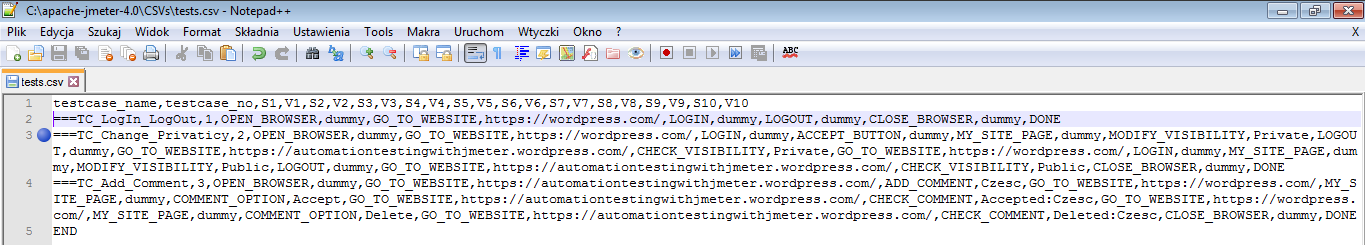
\includegraphics[width=1\textwidth]{NotePad.PNG}
\caption[Testy zapisane w pliku .csv - otwarte w programie Notepad++]{\label{fig:ham}Testy zapisane w pliku .csv - otwarte w programie Notepad++  \\ Źródło: opracowanie własne}
\end{figure}

\section{Uruchomienie testów}

Do uruchomienia testów należy otworzyć zainstalowanego wcześniej JMetera. Na rysunku 4.6 przedstawiono, jakie komendy do Wiersza poleceń na Windowsie należy wpisać, żeby otworzyć wersję graficzną JMetera, w której uruchamiamy plik \textit{Tests.jmx}. Zestaw testów został zapisany w pliku \textit{tests.csv}, do którego należy podać ścieżkę w CSV Config Element dla \textit{Tests.jmx}.

\begin{figure}[H]
\centering
\captionsetup{justification=centering}
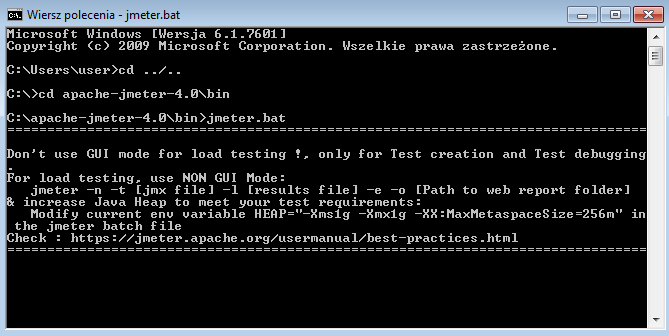
\includegraphics[width=1\textwidth]{testy_csv.png}
\caption[Sposób otworzenia JMetera - przez windowsowy wiersz poleceń]{\label{fig:ham}Sposób otworzenia JMetera - przez windowsowy wiersz poleceń \\ Źródło: opracowanie własne}
\end{figure}

\section{Wyniki wykonania testów}

Do zestawienia wyników wykonania testów w JMeterze wykorzystuje się komponent zwany \textit{Aggregate Report}, który tworzy wiersz tabeli dla każdego wykonanego kroku testowego. Zbiera informacje takie jak liczba wystąpień danego kroku, czas średni, maksymalny, minimalny wykonania czy wydajność mierzoną jako żądanie na sekundę. \cite{comp}

\begin{figure}[H]
\centering
\captionsetup{justification=centering}
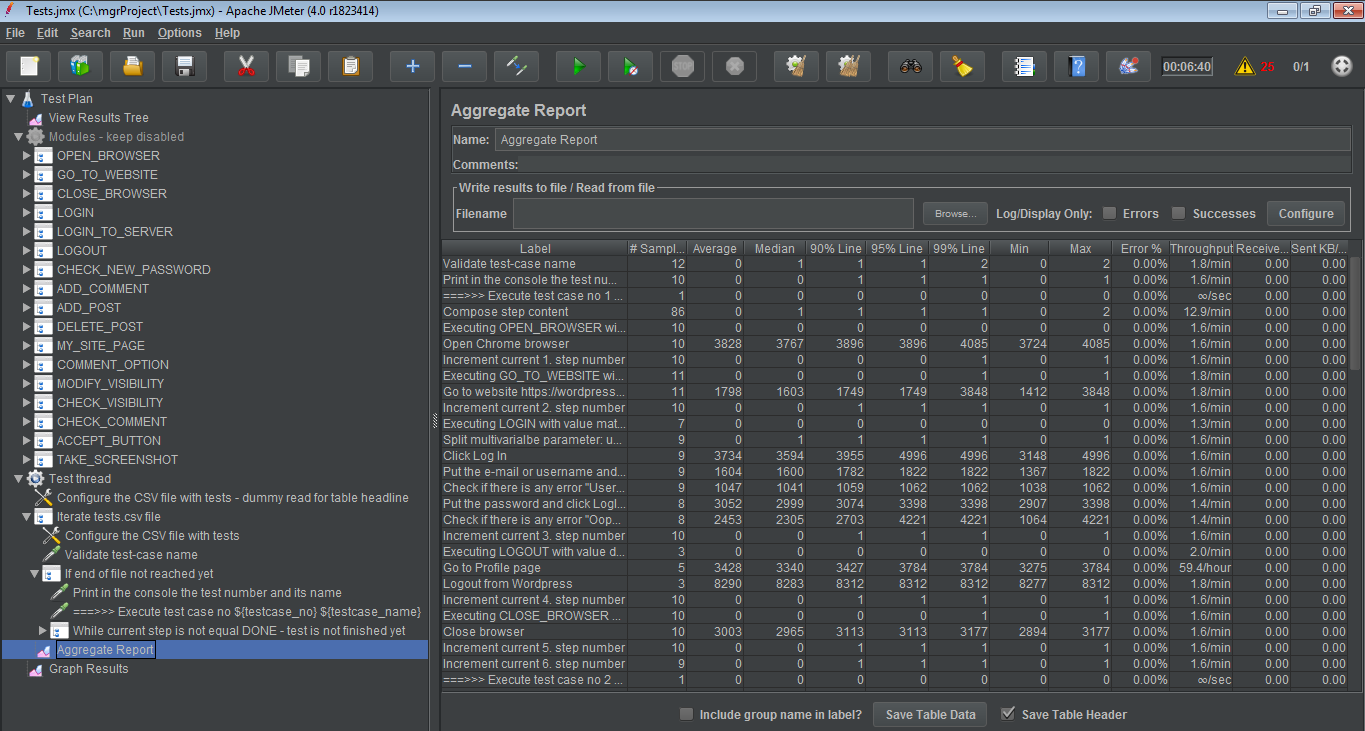
\includegraphics[width=1.05\textwidth]{aggr.PNG}
\caption[Rezultaty wykonania testów]{\label{fig:ham}Rezultaty wykonania testów \\ Źródło: opracowanie własne}
\end{figure}

Jak widać na powyższym rysunku, wykonanie dziesięciu testów zajęło łącznie 6 minut i 40 sekund, czyli średnio jeden test wykonał się w ciągu około 40 sekund.


Poniżej zostaną wyjaśnione parametry występujące w raporcie. Tutaj czasy są podawane w milisekundach.

\begin{itemize}
    \item \textit{Label} - Krok testowy
    \item \textit{\# Samples} - Liczba wystąpień dla tego samego kroku
    \item \textit{Average} - Średni czas wykonania zbioru rezultatów.
    \item \textit{Median} - Mediana czasu wykonania zbioru rezultatów.
    \item \textit{90\% Line} - percentyl 90\%, czyli wykonanie 90\% kroków testowych zajęło nie mniej niż podany czas.
    \item \textit{95\% Line} - percentyl 95\%, czyli wykonanie 95\% kroków testowych zajęło nie mniej niż podany czas.
    \item \textit{99\% Line} - percentyl 99\%, czyli wykonanie 99\% kroków testowych zajęło nie mniej niż podany czas.
    \item \textit{Min} - Najkrótszy czas wykonania dla kroków testowych o tej samej nazwie.
    \item \textit{Max} - Najdłuższy czas wykonania dla kroków testowych o tej samej nazwie
    \item \textit{Error \%} - Procent błędów występujących w żądaniach.
    \item \textit{Throughput} - wydajność mierzona w zapytaniach na sekundę, minutę czy godzinę.
    \item \textit{Received KB/sec} - wydajność mierzona w otrzymanych kilobajtach na sekundę.
    \item \textit{Sent KB/sec} - wydajność mierzona w wysłanych kilobajtach na sekundę.
\end{itemize}



\begin{figure}[H]
\centering
\captionsetup{justification=centering}
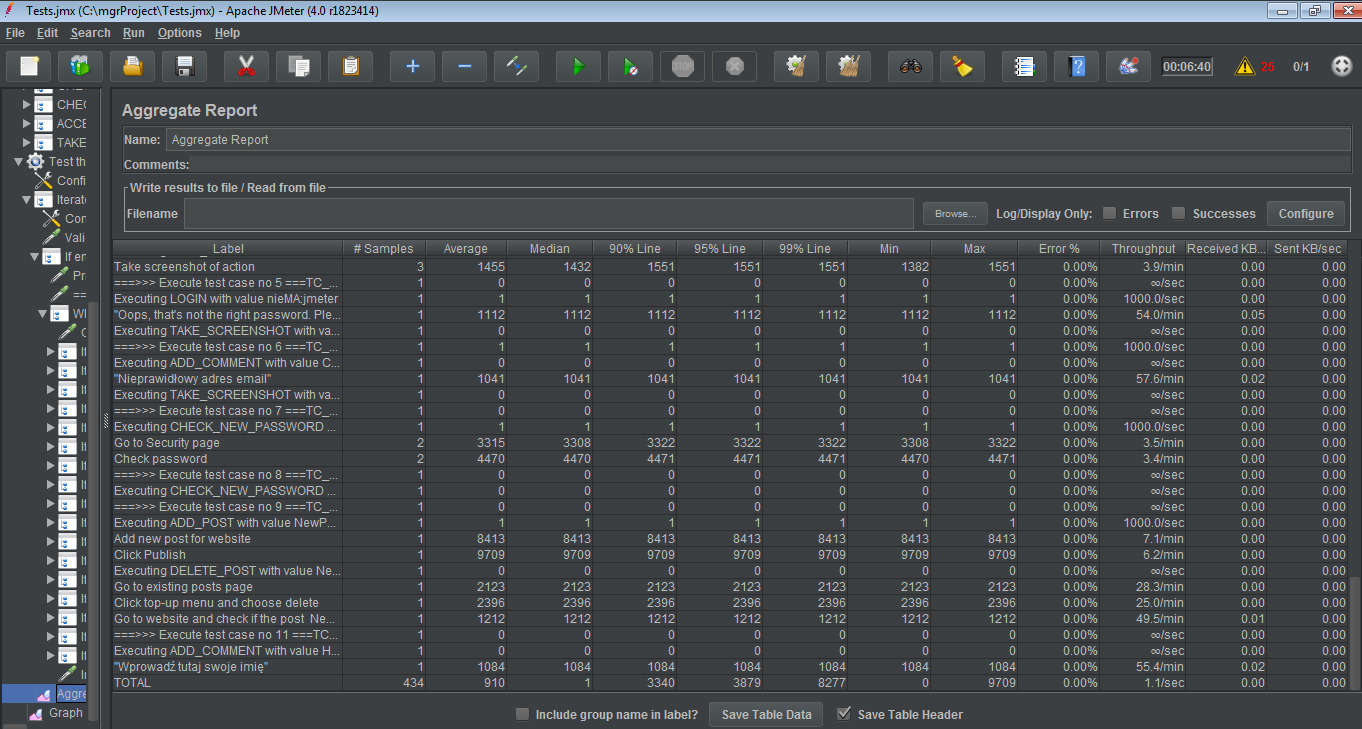
\includegraphics[width=1.05\textwidth]{aggregate.PNG}
\caption[Rezultat wykonania testów z wierszem TOTAL podsumowującym wszystkie kroki testowe]{\label{fig:ham}Rezultat wykonania testów z wierszem TOTAL podsumowującym wszystkie kroki testowe  \\ Źródło: opracowanie własne}
\end{figure}

Analizując otrzymane wyniki dla wiersza z wartością w kolumnie Label równą TOTAL, można wyciągnąć następujące wnioski:
\begin{itemize}
    \item Wystąpiło 434 kroków testowych.
    \item Średni czas wykonania każdego z nich wynosi 910 milisekundy, czyli niecałą sekundę.
    \item Mediana jest równa 1, czyli 434 kroków testowych wykonało się co najwyżej w 1 milisekundę, a pozostałe 90 kroków powyżej 1 milisekundy.
    \item 90\% kroków testowych, czyli 391, wykonuje się w co najwyżej 3340 milisekundach. Analogicznie, 412 kroków zakończy się do 3879 milisekund, a 430 - do 8.277 sekund.
    \item Najkrótszy czas wykonania kroku testowego to 0 milisekund (czyli istnieją takie, które nic nie wykonują), natomiast najdłuższy trwał 9.709 sekund.
    \item Procent błędów dla każdego kroku testowego jest równie 0, a to oznacza, że nie wykryto żadnych błędów podczas wykonania się testów.
    \item Średnia wydajność wynosi 1.1 zapytania na sekundę. Warto też zauważyć, że dla większości kroków testowych wydajność jest mierzona jako zapytanie na minutę, a dla niektórych jest ona równa $\inf$ na sekundę.
    \item Wydajność zarówno dla otrzymanych, jak i wysłanych kilobajtach na sekundach jest równa 0.
\end{itemize}


Wyniki otrzymane w Aggregate Report można zapisać w formie pliku .csv, klikając w przycisk \textit{Save Table Data}, który jest widoczny na samym dole na rysunkach 4.7. oraz 4.8.

\section{Określenie czasu odpowiedzi oraz zużycie zasobów po stronie serwera WordPressa}

W ramach części badawczej niniejszej pracy został wykonany również pomiar pamięci oraz CPU (zużycia procesora) po stronie serwera WordPressa względem czasu w sekundach podczas wykonania testu \textit{TC\_WordPress\_Server} dla 10, 25 oraz 100 użytkowników. Przeprowadzono test obciążeniowy, używając narzędzia JMeter wraz z Selenium do logowania się na stronę serweru, który znajdował się na stronie 
\newline
\textit{http://c8e2f540.ngrok.io/wp-login.php}.

\subsection{Zużycie pamięci}

\begin{figure}[H]
\centering
\captionsetup{justification=centering}
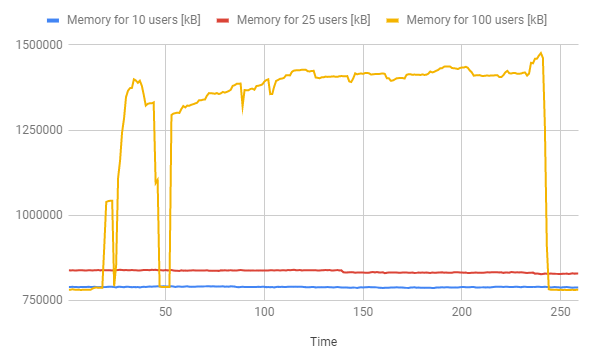
\includegraphics[width=1\textwidth]{Memory.PNG}
\caption[Zużycie pamięci serwera w kilobajtach względem czasu]{\label{fig:ham}Zużycie pamięci serwera w kilobajtach względem czasu  \\ Źródło: opracowanie własne}
\end{figure}

Zarówno jak dla dziesięciu, jak i dla dwudziestu pięciu użytkowników zużycie pamięci nie jest zauważalnie widoczne przy zadanym obciążeniu. Mają one podobne wartości, oscylujące około 800000 kilobajtów. 

Sytuacja jest inna przy testowaniu ruchu serwera dla 100 użytkowników - tutaj w czasie od 0 do 20 zużycie jest niemal takie same, jak w przypadku dziesięciu użytkowników, ale wzrasta między 20 a 22 sekundą do 1100000 kilobajtów. Chwilowo zauważalny jest spadek, by potem od 25 sekundy wzrosło do 1350000 KB. Po kolejnym spadku użycia pamięci między 30 a 49 sekundą następuje wzrost od czasu równego około 52, przez co zużycie pamięci waha się między 1300000 a 1450000 KB. Test kończy się po około 249 sekundach, dlatego w tym czasie zauważalny jest znaczący spadek do około 750000 KB. 

\subsection{Zużycie procesora (CPU)}

\begin{figure}[H]
\centering
\captionsetup{justification=centering}
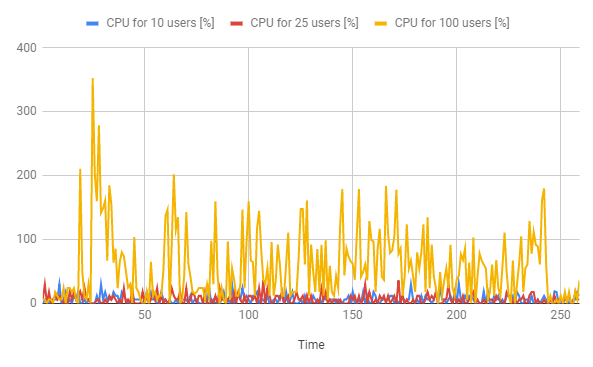
\includegraphics[width=1\textwidth]{CPU.PNG}
\caption[Pomiar zużycia procesora (w procentach) względem czasu (w sekundach)]{\label{fig:ham}Pomiar zużycia procesora (w procentach) względem czasu (w sekundach) \\ Źródło: opracowanie własne}
\end{figure}

Dla 100 użytkowników zużycie procesora między 20 a 22 sekundą wzrasta do ponad 200 \%, żeby chwilowo spaść, a następnie po raz kolejny wzrosnąć do 350 \% w 25 sekundzie. Następuje wtedy gwałtowny spadek do 0 \%. Od 50 do 249 zużycie utrzymuje się na poziomie między 50 a 200 \%.

W przypadku 10 oraz 25 użytkowników zużycie procesora nie przekracza 40 \%, czyli dla takiej liczby użytkowników obciążenie nie wpływa 

\newpage

\section{Wnioski}
Wykorzystanie rozwiązania omówionego w tym rozdziale niesie za sobą wiele korzyści. Jednym z nich jest wsparcie przez JMetera integracji z Selenium WebDriver, dzięki czemu można przeprowadzić automatyzację zarówno testów GUI, jak i aplikacji webowych. Oba narzędzia, jako że są zaimplementowane w Javie, pozwalają na napisanie testów end-to-end, wystawienie środowiska oraz przywrócenie stanu testów do początkowego.


JMeter jako narzędzie zbudowane w dużej mierze na wtyczkach może być rozszerzalne o dodatkowe wtyczki, co przykłada się na dokładniejsze sprawdzenie systemu. Można w nim też wykonać testy wydajnościowe dla istniejących scenariuszy, dodając tylko w Thread Group zwiększoną liczbę wątków.



